% Requires: \usepackage{graphicx}

\subsection{Downstream Client Case Study: FlowDroid}
\label{sec:downstream-flowdroid}

We further check whether FSpec can support an existing downstream taint-analysis client by running FlowDroid on OWASP Benchmark Java v1.2. This lightweight case study focuses on whether FlowDroid can consume FSpec-specialized points-to information without losing baseline-reported taint findings, while reducing downstream analysis cost.

\begin{figure*}[t]
\centering
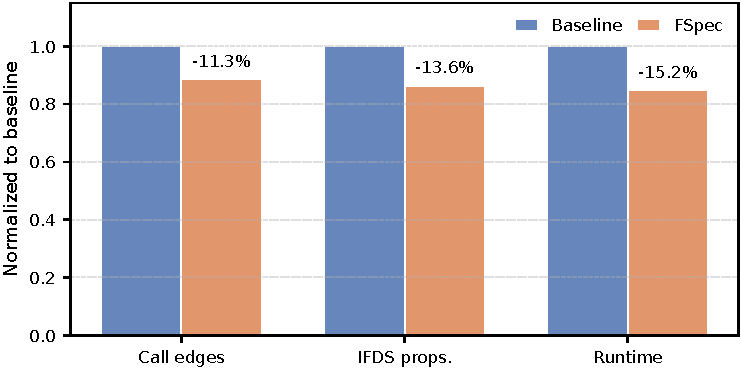
\includegraphics[width=0.95\textwidth]{data/FlowDroid.pdf}
\caption{FSpec's impact on the paired OWASP/FlowDroid runs. FSpec retains all baseline-reported FlowDroid findings and reduces the projected call graph, IFDS propagation workload, and aggregate end-to-end runtime.}
\label{fig:flowdroid-deltas}
\end{figure*}

Figure~\ref{fig:flowdroid-deltas} summarizes the main quantitative effect. Across the completed paired OWASP batches, every taint finding reported by the baseline FlowDroid run is still reported with FSpec. Meanwhile, the projected call graph used by FlowDroid is reduced in every evaluated category, with an 11.33\% aggregate reduction. FlowDroid's IFDS edge-propagation count decreases by 13.61\%, and end-to-end runtime improves by 15.19\% on the paired subset. These results support the intended downstream use case, showing that FSpec can support FlowDroid without missing baseline-reported taint findings while reducing the overall analysis space and aggregate runtime.

As a limitation, this case study reports a subset of 641 completed paired OWASP batches under our experimental budget, rather than the full OWASP/FlowDroid benchmark. Batches with timeout, OOM, or abnormal FlowDroid termination are excluded from the paired comparison.
